%%%%%%%%%%%%%%%%%%%%%%%%%%%%%%%%%%%%%%
% One Column
%%%%%%%%%%%%%%%%%%%%%%%%%%%%%%%%%%%%%%
\documentclass[smallabstract,smallcaptions]{dccpaper}

\usepackage{epsfig}
\usepackage{epstopdf}
\usepackage{citesort}
\usepackage{amsmath}
\usepackage{amssymb}
\usepackage{color}
\usepackage{url}

\newlength{\figurewidth}
\newlength{\smallfigurewidth}


%%%%%%%%%%%%%%%%%%%%%%%%%%%%%%%%%%%%%%
% One Column
%%%%%%%%%%%%%%%%%%%%%%%%%%%%%%%%%%%%%%
\setlength{\smallfigurewidth}{2.75in}
\setlength{\figurewidth}{6in}

\begin{document}

\title
{\large
\textbf{Universal Rate-Distortion Analysis for Various Source Distributions}
}

\author{%
Shengbin Meng, Jun Sun$^{\ast}$, Yizhou Duan, and Zongming Guo\\[0.5em]
{\small\begin{minipage}{\linewidth}\begin{center}
\begin{tabular}{ccc}
Institution of Computer Science and Technology, \\
Peking University, Beijing, 100086, China\\
\url{{mengshengbin, sunjun, duanyizhou, guozongming}@pku.edu.cn}
\end{tabular}
\end{center}\end{minipage}}
}

\maketitle
\thispagestyle{empty}

\begin{abstract}
This paper studies the complex Rate-Distortion (R-D) analysis problem from a universal perspective. For various probability distributions that have been used to describe real source signals, common properties and principles are revealed and validated based on the popular dead-zone plus uniform threshold scalar quantization with nearly-uniform reconstruction quantizer (DZ+UTSQ/NURQ) scheme. First, properties of R-D function are investigated through its derivative. It is mathematically proved that, for any source distribution that can be expressed as the product of a Scaling Factor (SF) and its remaining part, SF does not affect the derivative of its R-D function. Second, finer and efficient DZ+UTSQ/NURQ design principles are deduced for various sources, which can be used to conveniently guile the parameter selection of practical quantizers and evaluate the R-D performance of them. Simulation experiments for Cauchy distribution, which still lacks thorough analysis in the literature, are present to conform the universal findings.
\end{abstract}

\section{Introduction}

\let\thefootnote\relax\footnotetext{* is the corresponding author.}

The lossy compression of digital video/image data finally leads to transform-based coding of residuals obtained from intra or inter-frame prediction \cite{Sullivan_IEEE2005}. The coefficients of the transform (generally DCT or alike), are processed through quantization and entropy coding, from which bits are produced and distortion is introduced. The rate of bits coming from the entropy coder and the distortion caused by quantization are two aspects that measure the efficiency of the compression. In this scenario, the transform coefficients are referred to as source signal, and the whole process belongs to the source coding realm.

As one of the fundamental issues of source coding, rate-distortion (R-D) analysis has attracted considerable research attentions. R-D analysis focuses on studying the essential relationship between rate and distortion of the source signal under applicable quantization technologies. In practice, a source signal is typically characterized by its probability distribution, whereas the transform-based entropy-constrained scalar quantization is the most extensively applied quantization technology \cite{Hang_TCSVT1997}. Therefore, R-D analysis is generally represented by studying the R-D relationship and R-D performance of applying certain scalar quantizer to a given source distribution.

On one hand, to evaluate the best attainable R-D performance, for some given source distributions, different types of scalar quantizers have been analyzed and compared \cite{Sullivan_TIT1996}, among which the dead-zone plus uniform threshold scalar quantizer (DZ+UTSQ) with nearly-uniform reconstruction quantizer (NURQ) is recommended and now applied in all major international video/image coding standards \cite{Sullivan_VCIP2005}. On the other hand, regards to which distribution is most appropriate to statistically characterize the real source signal (DCT coefficients), no consensus is ever reached. Some researchers prefer Gaussian, Laplacian, or their parametric family Generalized Gaussian distribution (GGD) \cite{Pratt_Wiley1978,Smooth_SPIE1996,Sun_TCSVT2009}, while others claim that Cauchy distribution is a better choice \cite{Kamaci_TCSVT2005} \cite{Rod_TCSVT2010}. Proposals for more sophisticated distributions such as mixed Gaussian \cite{Eude_ICASSP1994}, Bernoulli GGD \cite{Fraysse_TIT2009}, multiple Laplacian \cite{Lee_TCSVT2014} are also reported. Among these various distributions, R-D analysis for the Gaussian family has been thoroughly conducted \cite{Sun_TIP2013}. For example, performance of the DZ+UTSQ/NURQ quantizer is clearly shown for Laplacian and Gaussian by Gary in \cite{Sullivan_VCIP2005}. However, for Cauchy and other more complex distributions, the existing conclusions are still quite limited and are mostly based on empirical approach which may lack accuracy and robustness.

In this paper, instead of focusing on the R-D analysis of a specific source distribution, we try to reveal the common rules existing for a variety of different source distributions. The main contribution of this study is to provide insights and assistance in R-D modeling and quantizer design for real coding applications, regardless of the distribution form of the source. First, R-D properties for general sources under DZ+UTSQ/NURQ are investigated to identify the irrelevance of source scaling factor to the derivative R-D function, which properly reduces the complexity of the R-D modeling problem. Second, by taking the revealed properties into account, efficient DZ+UTSQ/NURQ design principles are deduced for various sources, which can be used to conveniently guide the parameter selection of practical quantizers and evaluate the R-D performance of them. The general findings are validated with the Cauchy distribution, and are also consistent with existing conclusions of other distributions.

The rest of this paper is organized as follows. In Section \ref{sec:background}, the background knowledge of our analysis is briefly introduced. On this basis, Section \ref{sec:property} and Section \ref{sec:principle} respectively discusses the general R-D properties and quantizer design principles that apply to various source distributions, with both mathematical derivation and simulated validation. Finally, concluding remarks are given in Section \ref{sec:conclusion}.

\section{Background Knowledge}
\label{sec:background}

\subsection{Scaling Factor of Source Distributions}

Let $p(x)$ be the Probabilistic Density Function (PDF) of an arbitrarily given source distribution, and $c>0$ is one of its parameters. If there exists a function $q(x)$ irrelevant to $c$ satisfying:
\begin{equation}
\label{equ:SF}
p(x)=\frac{1}{c} q(\frac{x}{c}),\qquad \forall x \in \mathbf{R},
\end{equation}
the parameter $c$ is defined as a \emph{Scaling Factor} (SF) of $p(x)$, and $q(x)$ is defined as the \emph{Remaining Part} (RP) irrelevant to $c$.

According to (\ref{equ:SF}), typical zero-mean source distributions such as GGD, Generalized Cauchy Distribution (GCD) and Cauchy are expressed in terms of SF and RP in Table \ref{tab:SF}. Note that, GGD becomes Laplacian and Gaussian when $\alpha=1.0$ and $\alpha=2.0$, and Cauchy is a special case of GCD with $k=2.0$.

\begin{table*}
	\begin{center}
	\caption{\label{tab:SF}%
	The SF and RP of Some Typical Zero-Mean Source Distributions}
	\begin{minipage}{0.95\linewidth}
		\renewcommand{\arraystretch}{1.7}
		\begin{tabular}{cccc}
			Source Distribution & PDF: $p(x)$ & SF: $c$ & RP: $q(x)$ \\
			\hline
			GGD & $\frac{g_1(\alpha)}{\beta}\exp\left(-\left(g_2(\alpha)\frac{|x|}{\beta}\right)^\alpha\right)$ & $\beta$ & $g_1(\alpha)\exp\left(-\left(g_2(\alpha)|x|\right)^\alpha\right)$ \\
			GCD & $\frac{k\Gamma(\frac{2}{k})}{2(\Gamma(\frac{1}{k}))^2} h\left(h^k + |x|^k\right)^{-\frac{2}{k}}$ & $h$ & $\frac{k\Gamma(\frac{2}{k})}{2(\Gamma(\frac{1}{k}))^2} \left(1+|x|^k\right)^{-\frac{2}{k}}$ \\
			Cauchy & $\frac{1}{\pi} \frac{\mu}{\mu^2+x^2}$ &  $\mu$ & $\frac{1}{\pi (1+x^2)}$ \\
			\hline
		\end{tabular}
		\let\thefootnote\relax\footnotetext{$g_1(\alpha)=\frac{\alpha\cdot\Gamma(3/\alpha)^{1/2}}{2\cdot\Gamma(1/\alpha)^{3/2}}$, and $g_2(\alpha)=\left[{\frac{\Gamma(3/\alpha)}{\Gamma(1/\alpha)}}\right]^{1/2}$.}
	\end{minipage}
	\end{center}
\end{table*}

\subsection{DZ+UTSQ/NURQ Scheme}

The widely used DZ+UTSQ/NURQ scheme \cite{Sullivan_VCIP2005} is illustrated in Fig. \ref{fig:DZ+UTSQ_NURQ}, which consists of DZ+UTSQ classification process and NURQ reconstruction process, both symmetric about zero. In classification, each input signal is rounded to an integer quantization index according to its \emph{quantization interval} $I$, which is determined by the \emph{quantization threshold} $T$. Then in reconstruction, each quantization index is mapped to a \emph{reconstruction value} $R$. For the quantization index $k$, the corresponding $kth$ quantization interval $I_{k}$ of general DZ+UTSQ/NURQ is denoted by:
\begin{equation}
\label{equ:interval}
I_{k}=\left\{ \begin{array}{ll}
(T_{-1}, T_{1}),         & k = 0 \\
{[T_{k}, T_{k+1})},        & k \ge 1 \\
(T_{-k-1}, T_{-k}],      & k \le -1
\end{array}\right. .
\end{equation}
The quantization threshold $T_{k}$ and the reconstruction value $R_{k}$ are expressed as:
\begin{equation}
\label{equ:DZ+UTSQ/NURQ}
T_{k}=\left\{ \begin{array}{ll}
(k-1+z)s, & k \ge 1 \\
-T_{-k},  & k \le -1
\end{array}\right.
\qquad \textrm{and} \qquad
R_{k}=\left\{ \begin{array}{ll}
0,        & k = 0 \\
(k+f)s,   & k \ge 1 \\
-R_{-k},  & k \le -1
\end{array}\right. ,
\end{equation}
where $z$ is half of the dead-zone size, and $f$ is the offset between the reconstruction value and the inner threshold of the quantization interval, both normalized by the quantization step size $s$. Almost all of quantizers in practice belong to this DZ+UTSQ/NURQ scheme (for example, H.264/AVC video coding standard uses a uniform reconstruction quantizer which is a special case of DZ+UTSQ/NURQ with $f=0$), therefore our work based on DZ+UTSQ/NURQ is quite important and useful.

\begin{figure}[tp]
\centering
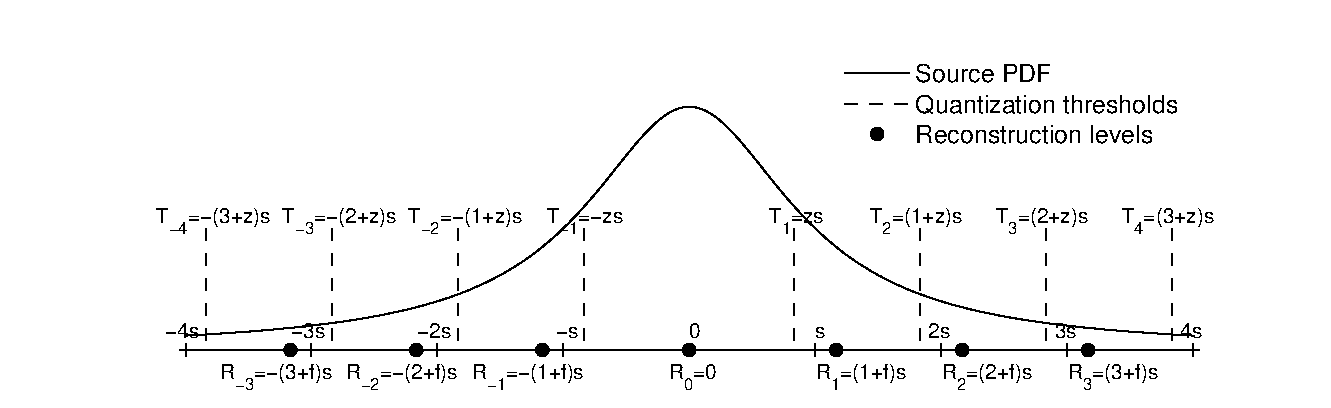
\includegraphics[width = 1.0\linewidth]{Figures/section2/DZ+UTSQ_NURQ}\\
\caption{\label{fig:DZ+UTSQ_NURQ}%
Illustration of DZ+UTSQ/NURQ Scheme.}
\vspace{5pt}
\end{figure}

\subsection{Problem Formulation of R-D Analysis}

Consider an input random variable $X$ of distribution $p(x)$ being quantized with the DZ+UTSQ/NURQ scheme. After the DZ+UTSQ classification process, the output entropy of the quantizer, which is also the bit rate required to encode the output values, can be denoted by the \emph{R-Q function} (RQF):
\begin{equation}\label{equ:formula-rq}
	R(z, s) = -\sum_{k=-\infty}^{+\infty} P_k \log_2 P_k ,
\end{equation}
where $P_k$ is the possibility of the output value being quantization index $k$, or equivalently, the input value lying in quantization interval $I_{k}$:
\begin{equation}\label{equ:formula-pk}
	P_k = P\{X \in I_k\} =
	\begin{cases}
		\int_{-z s}^{z s} p(x) dx
		= 2 \int_{0}^{z s} p(x) dx,
		& k=0 \\
		\int_{(k-1+z) s}^{(k+z) s} p(x) dx,
		& k \ge 1 \\
		P_{-k},
		& k \le -1 .
	\end{cases}
\end{equation}  

Likewise, after the NURQ reconstruction process, the distortion, using mean squared error (MSE) as criterion, can be denoted by the \emph{D-Q function} (DQF):
\begin{equation}\label{equ:formula-dq}
	D(z, s, f) =\sum_{i=-\infty}^{+\infty} E_k
\end{equation}
where $E_k$ is the reconstruction error generated in quantization interval $I_k$:
\begin{equation}\label{equ:formula-dk}
	E_k=
	\begin{cases}
		\int_{-z s}^{z s} |x|^2 p(x) dx,
		& k=0 \\
		\int_{(k-1+z) s}^{(k+z) s} |x - (k+f) s|^2 p(x) dx,
		& k \ge 1 \\
		E_{-k},
		& k \le -1 .
	\end{cases}
\end{equation}

The RQF and DQF provide a way to calculate rate and distortion, and by combining the two, we can define a \emph{R-D function} $R=f(D)$, or its inverse $D=f(R)$, to represent the R-D relationship in source coding. However, for most source distributions, the sophisticated PDFs (e.g. the exponential form for GGD and power form for Cauchy) make it difficult or impossible to directly obtain the closed-form RQF and DQF from (\ref{equ:formula-rq}) - (\ref{equ:formula-dk}), not to mention deriving the accurate R-D function. In the following sections, we reveal the universal properties and principles that does not require exact formula of PDF or R-D function, to assist the R-D analysis of various source distributions.

\section{Universal Properties of R-D Function Under DZ+UTSQ/NURQ}
\label{sec:property}

In this section, we try to investigate the properties of R-D function from its derivate, bypassing the obstructing fact that formula of R-D function for a non-trivial source distribution is generally not available.

Based on our observation and analysis, it is revealed that, for any source distribution that can be expressed as the product of a SF and its RP, the SF does not affect its derivative R-D function under the DZ+UTSQ/NURQ scheme. Next, we first give mathematical deduction and proof of this universal property, then validate it with the specific distribution of Cauchy by presenting some simulation results.

\subsection{Mathematical Deduction and Proof}

For any given source distribution satisfying (\ref{equ:SF}), the original PDF $p(x)$ can be expressed as the product of a SF $c$ and RP $q(x)$. Then for quantization step size $s$, we can find a value $\delta$ such that $s=c \cdot \delta$. By replacing $p(x)$ with $1/c \cdot q(x/c)$ and $s$ with $c \cdot \delta$, the RQF and DQF can be expressed in a new form. First, for RQF, (\ref{equ:formula-pk}) can be rewritten as:
\begin{equation}\label{equ:formula-pknew}
	P_k =
	\begin{cases}
		\int_{-z c\delta}^{z c\delta} q\left(\frac{x}{c}\right) d\left(\frac{x}{c}\right)
		= 2 \int_{0}^{z \delta} q(x) dx,
		& k=0 \\
		\int_{(k-1+z) c\delta}^{(k+z) c\delta} q\left(\frac{x}{c}\right) d\left(\frac{x}{c}\right)
		=\int_{(k-1+z) \delta}^{(k+z) \delta} q(x) dx,
		& k \ge 1 \\
		P_{-k},
		& k \le -1 ,
	\end{cases}
\end{equation} 
which becomes a function of $\delta$ and $z$. Substitute (\ref{equ:formula-pknew}) into (\ref{equ:formula-rq}), and the RQF also becomes a function of $\delta$ and $z$. Specifically, given the constant dead-zone ratio $z$, the rate is just a function of $\delta$: 
\begin{equation}\label{equ:formula-rqnew}
	R = R_z(\delta).
\end{equation}

Similarly, for DQF, (\ref{equ:formula-dk}) can be rewritten as:  
\begin{equation}\label{equ:formula-dknew}
	E_k =
	\begin{cases}
		\int_{-z c\delta}^{z c\delta} |x|^2 q\left(\frac{x}{c}\right) d\left(\frac{x}{c}\right)
		= c^2\int_{-z \delta}^{z \delta} |x|^2 q(x) d(x),
		& k=0 \\
		\int_{(k-1+z) c\delta}^{(k+z) c\delta} |x - (k+f) c\delta|^2 q\left(\frac{x}{c}\right) d\left(\frac{x}{c}\right)\\
		=c^2\int_{(k-1+z) \delta}^{(k+z) \delta} |x - (k+f) \delta|^2 q(x) dx,
		& k \ge 1 \\
		E_{-k},
		& k \le -1 .
	\end{cases}
\end{equation} 
For convenience, we define $F_k$ as:
\begin{equation}\label{equ:formula-fk}
	F_k =
	\begin{cases}
		= \int_{-z \delta}^{z \delta} |x|^2 q(x) d(x),
		& k=0 \\
		=\int_{(k-1+z) \delta}^{(k+z) \delta} |x - (k+f) \delta|^2 q(x) dx,
		& k \ge 1 \\
		F_{-k},
		& k \le -1 .
	\end{cases}
\end{equation}
Thus, we have $E_k = c^2 F_k$, where $F_k$ is only a function of $\delta, z$ and $f$, being irrelevant to $c$. Then according to (\ref{equ:formula-dq}), the distortion using MSE criteria is expressed as:
\begin{equation}\label{equ:formula-dqnew}
	D = c^2 \sum_{k=-\infty}^{+\infty} F_k, 
\end{equation}

In practice, another widely used distortion criteria is peak signal-to-noise ratio (PSNR), defined via MSE as $\textrm{PSNR} = 10 \log_{10}\left(\frac{MAX^2}{D}\right)$, where $MAX$ is a constant (the maximum signal value). We claim that, the derivative of D-R function $\textrm{PSNR}=f(R)$, i.e., $\frac{\partial\textrm{PSNR}}{\partial R}$ is irrelevant to $c$. It can be proved based on (\ref{equ:formula-rqnew}), (\ref{equ:formula-fk}), and (\ref{equ:formula-dqnew}), as follows.

With the definition of PSNR and (\ref{equ:formula-dqnew}), we have:

\begin{eqnarray*}
\frac{\partial\text{PSNR}}{\partial\delta}
&=&\frac{\partial}{\partial\delta}10 \log_{10}\left(\frac{MAX^2}{D}\right)
=-10\frac{\partial}{\partial\delta}\log_{10}D
=\frac{-10}{\ln{10}}\frac{1}{D}\frac{\partial D}{\partial\delta}
\\&=&\frac{-10}{\ln{10}}\frac{1}{c^2 \sum_{k=-\infty}^{+\infty} F_k}\frac{\partial}{\partial\delta} \left(c^2 \sum_{k=-\infty}^{+\infty} F_k\right)
\\&=&\frac{-10}{\ln{10}}\frac{1}{\sum_{k=-\infty}^{+\infty} F_k}\sum_{k=-\infty}^{+\infty} \frac{\partial F_k}{\partial\delta} .
\end{eqnarray*}

It can be seen that, $c$ is eliminated in the reduction and only $F_k$ is left. According to (\ref{equ:formula-fk}), $F_k$ is irrelevant to $c$, therefore $\frac{\partial\textrm{PSNR}}{\partial\delta}$ is irrelevant to $c$. From (\ref{equ:formula-rqnew}), it's easy to know that $\frac{\partial\textrm{R}}{\partial\delta}$ is also irrelevant to $c$. Based on the derivative method for compound functions, we have $\frac{\partial\textrm{PSNR}}{\partial R} = \frac{\partial\textrm{PSNR}}{\partial\delta}/\frac{\partial R}{\partial\delta}$. Since the numerator and denominator are both irrelevant to $c$, $\frac{\partial\textrm{PSNR}}{\partial R}$ is proved to be irrelevant to $c$.

\subsection{Validation}

The irrelevance of SF to the derivative of PSNR-R function is proved to be a universal property applicable to any source distribution satisfying (\ref{equ:SF}), including GGD and Cauchy which are commonly-used to model real video and image source signals. For GGD, in our previous work \cite{Sun_TCSVT2009}, the fact that its SF $\beta$ does not affect the derivative PSNR-R function is confirmed via extensive experimental results. For Cauchy distribution, under DZ+UTSQ/NURQ scheme, the curves of PSNR-R function and its derivative are drawn using simulated data and numerical methods, as illustrated in Fig. \ref{fig:RD_mu}. From Fig. \ref{fig:RD_mu}(a) and Fig. \ref{fig:RD_mu}(b) it can be seen that the PSNR-R curves corresponding to four SF values $\mu = 0.1, 0.2, 0.5, \; \textrm{and} \;0.8$ are of the same shape (parallel to each other); and Fig. \ref{fig:RD_mu}(c) and Fig. \ref{fig:RD_mu}(d) show that they have the same derivative.

Since the universal property holds true even when the distribution of the source cannot be clearly defined or all parameters of a distribution are not known, the complexity of R-D analysis in real coding applications can be properly reduced.

\begin{figure}[tp]
\begin{center}
\begin{tabular}{cc}
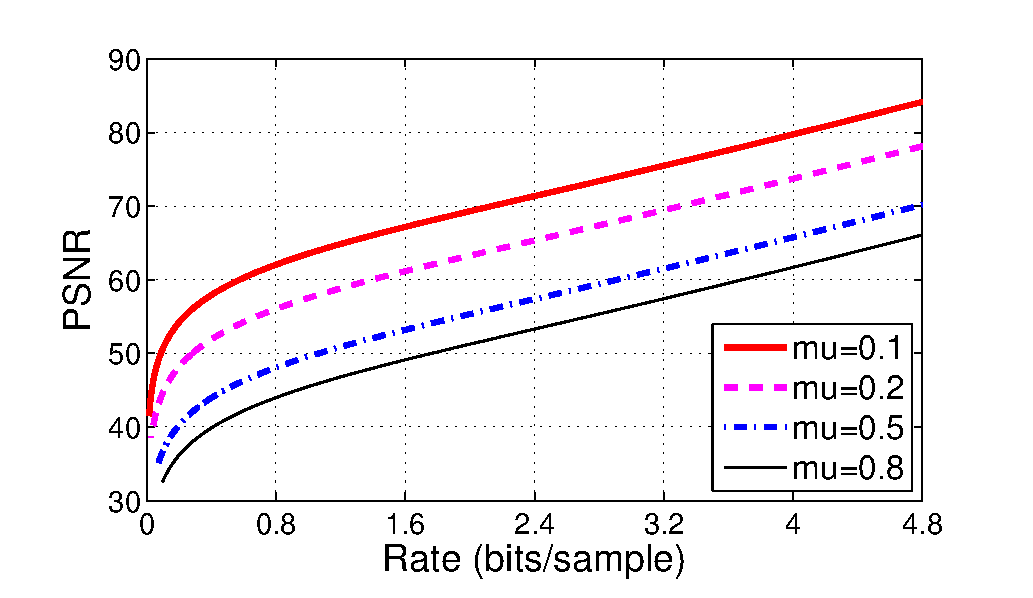
\includegraphics[width = 0.5\linewidth]{Figures/section3/RD_Cauchy_z=0_75_p=0} &
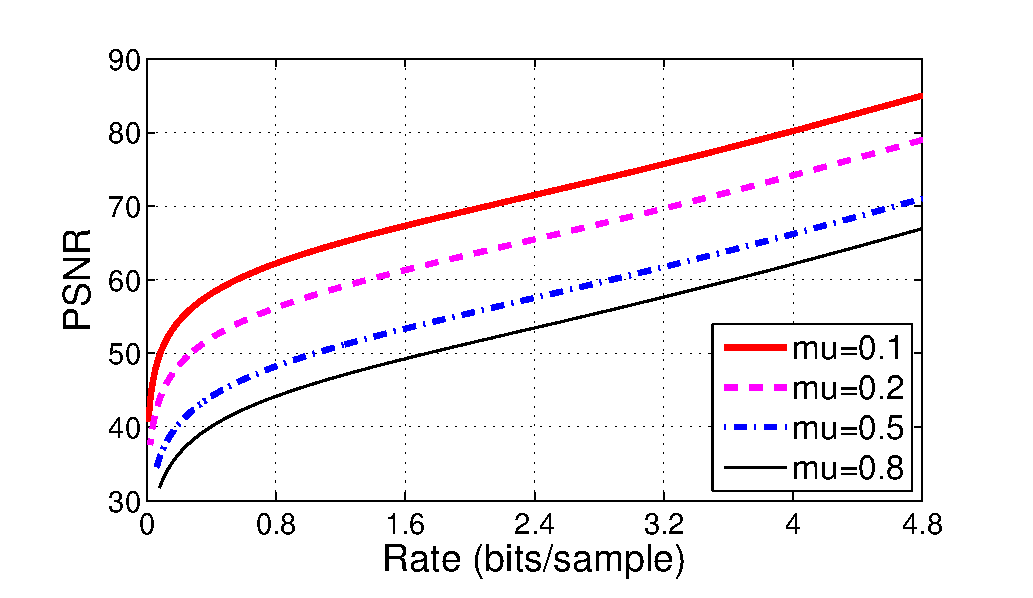
\includegraphics[width = 0.5\linewidth]{Figures/section3/RD_Cauchy_z=1_p=0_5} \\
{\small (a) $z=3/4,\;f=0$} & {\small (b) $z=1,\;f=1/2$} \\
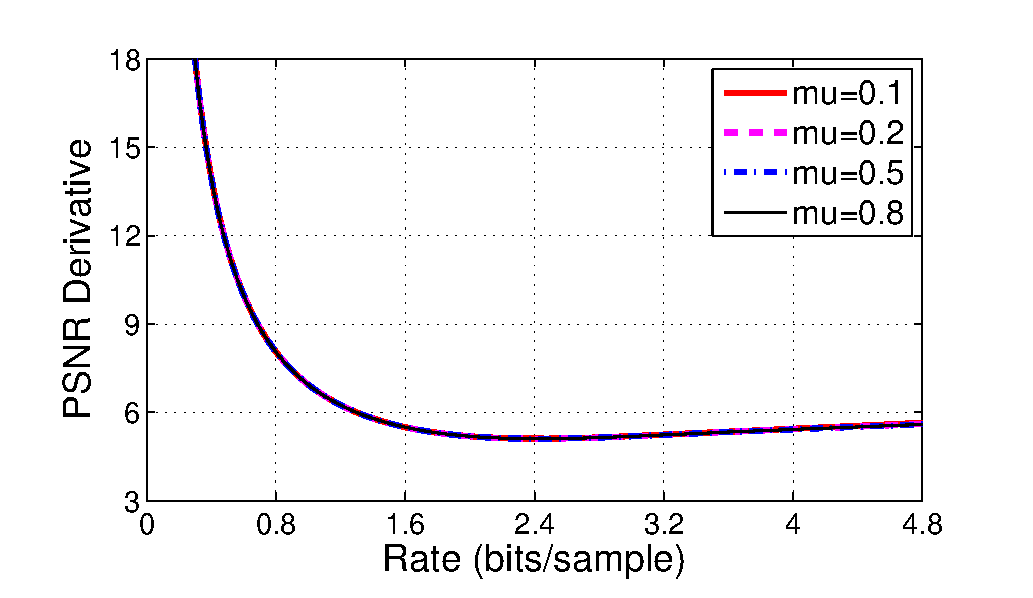
\includegraphics[width = 0.5\linewidth]{Figures/section3/RDDerivative_Cauchy_z=0_75_p=0} &
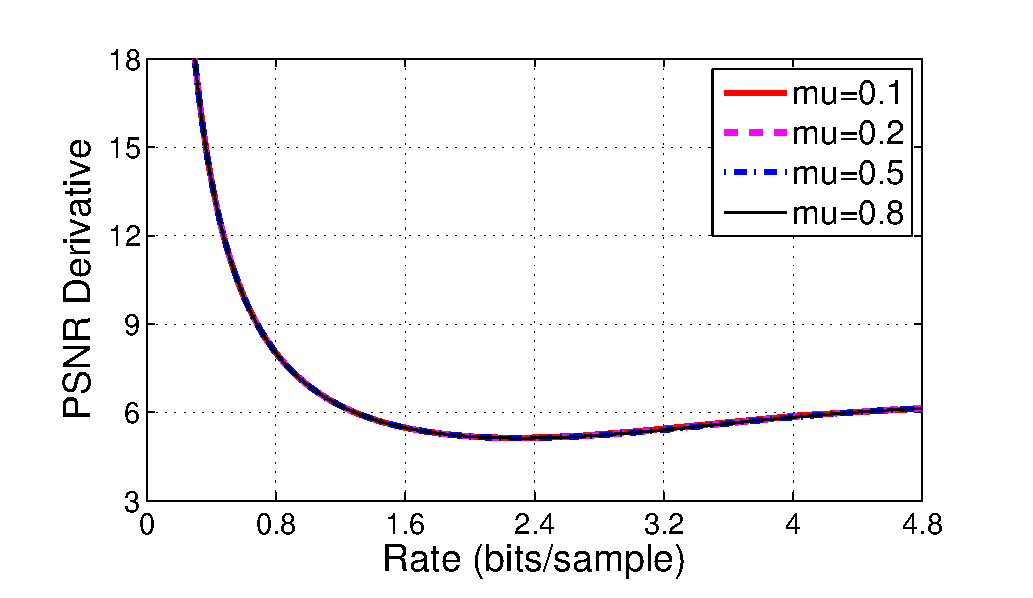
\includegraphics[width = 0.5\linewidth]{Figures/section3/RDDerivative_Cauchy_z=1_p=0_5} \\
{\small (c) $z=3/4,\;f=0$} & {\small (d) $z=1,\;f=1/2$}
\end{tabular}
\end{center}
\vspace{-20pt}
\caption{\label{fig:RD_mu}
Curves of PSNR-R function and its derivative for different $\mu$ of Cauchy distribution under DZ+UTSQ/NURQ.}
\end{figure}


\section{Efficient DZ+UTSQ/NURQ Design Principles for Various Sources}
\label{sec:principle}

The necessary conditions for a scalar quantizer to achieve optimum R-D performance were formulated in \cite{Farvardin_TIT1984}. Specifically, under MSE criterion, Max \cite{Max_TIT1960} obtained the famous conclusion that, for each quantization index $k$, the reconstruction level $R_k$ should be located at the \emph{centroid} of the PDF $p(x)$ within quantization interval $I_k$. Thus, for symmetric DZ+UTSQ/NURQ scheme, the optimum design requires:
\begin{equation}\label{equ:formula-OptQuant}
	{R_k}^* = \int_{(k-1+z)s}^{(k+z)s} xp(x)dx / \int_{(k-1+z)s}^{(k+z)s} p(x)dx, \quad k \ge 1,
\end{equation}
whereas for $k \le 0$ the results can be similarly deduced without loss of generality.

Based on (\ref{equ:formula-OptQuant}), we now deduce the necessary constraint on $z$ and $f$ for DZ+UTSQ/NURQ design to achieve optimum R-D performance.

First, for all types of distributions, the preliminary constraint on $z$ and $f$ should be:
\begin{equation}\label{equ:formula-PreConstraint}
	 0 < z - f \le 1. 
\end{equation}

Then we narrow the source distribution types to the widely-used source models of the real video/image signals. For these sources, the PDF is always zero-mean and monotonically decreasing in positive axis. With this feature, it is easy to prove:
\begin{equation}\label{equ:formula-Inequity1}
	\int_{(k-1+z)s}^{(k+z)s} xp(x)dx \le (k+z-\frac{1}{2}) s \int_{(k-1+z)s}^{(k+z)s} p(x)dx, \quad k \ge 1.
\end{equation}
By integrating (\ref{equ:formula-OptQuant}) and (\ref{equ:formula-Inequity1}), it is clear that:
\begin{equation}\label{equ:formula-Inequity2}
	{R_k}^* \le (k+z-\frac{1}{2}), \quad k \ge 1.
\end{equation}
From (\ref{equ:DZ+UTSQ/NURQ}) and (\ref{equ:formula-Inequity2}), the preliminary constraint (\ref{equ:formula-PreConstraint}) can be refined as:
\begin{equation}\label{equ:formula-RefConstraint}
	\frac{1}{2} \le z - f \le 1. 
\end{equation}

\begin{figure}[tp]
\begin{center}
\begin{tabular}{cc}
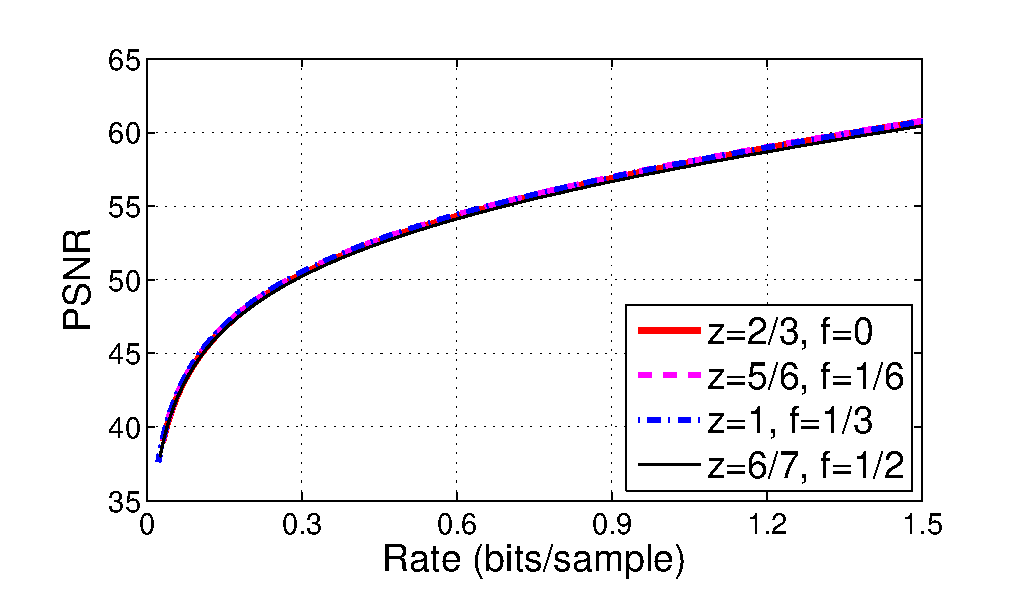
\includegraphics[width = 0.5\linewidth]{Figures/section4/RD_Cauchy_mu=0_5_z=p+0_67} &
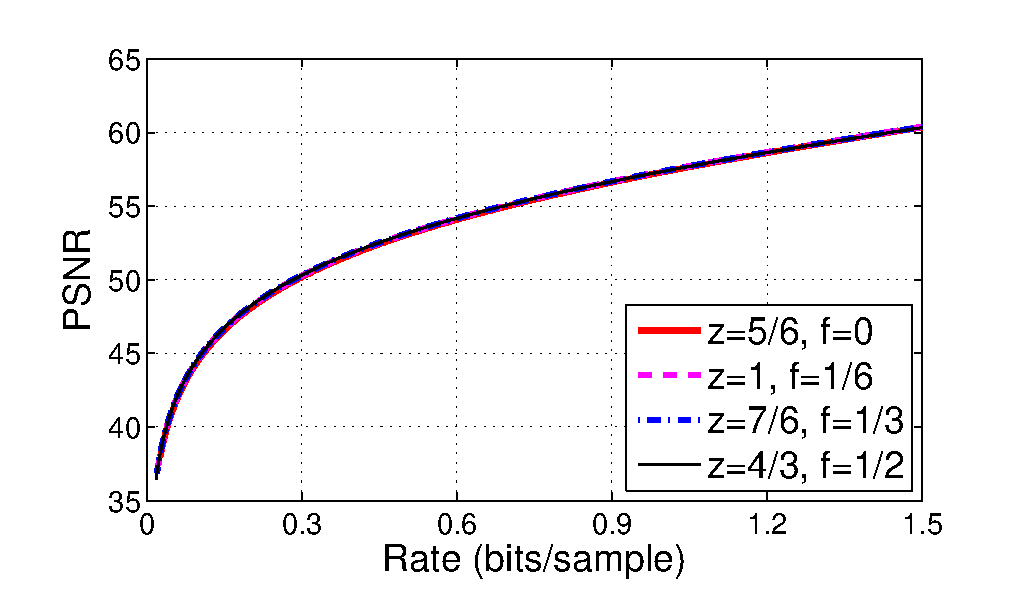
\includegraphics[width = 0.5\linewidth]{Figures/section4/RD_Cauchy_mu=0_5_z=p+0_83} \\
{\small (a) $z=p+2/3$} & {\small (b) $z=p+5/6$} 
\end{tabular}
\end{center}
\vspace{-20pt}
\caption{\label{fig:RD_same_pattern}
R-D performance comparison of different quantizer designs conforming to the same DZ+UTSQ/NURQ linear pattern satisfying (\ref{equ:formula-LinearConstraint}) for Cauchy $\mu=0.5$.}
\end{figure} 

Particularly, when the source distribution types are further specified as some zero-mean heavy-tailed distribution \footnote{http://en.wikipedia.org/wiki/Heavy-tailed\_distribution}, e.g. Cauchy distribution, the refined constraint (\ref{equ:formula-RefConstraint}) can be more accurately described. Consider the quantization interval $I_k$ ($k > 0$), where the reconstruction level $R_k$ divides $I_k$ into two parts: $\overline{T_k R_k}$ and $\overline{R_k T_{k+1}}$. Since Cauchy distribution provides a useful model of broad-tailed stochastic phenomena \cite{Farvardin_TIT1984}, in quantization intervals other than dead-zone ($\forall I_k, \; k \ne 0$), the PDF of Cauchy distribution can be precisely approximated as a straight line. Thus, when the slope of PDF in $I_k$ is fixed, according to the necessary condition (\ref{equ:formula-OptQuant}), to keep $R_k$ the centroid of PDF in $I_k$, the distance ratio of $\overline{T_k R_k} / \overline{R_k T_{k+1}}$ should remain constant. To make it clear, efficient DZ+UTSQ/NURQ design requires two different patterns $z_1, f_1$ and $z_2, f_2$ to satisfy:
\begin{equation}\label{equ:formula-ratio}
\frac{(k+f_1)-(k-1+z_1)}{(k+z_1)-(k+f_1)} = \frac{(k+f_2)-(k-1+z_2)}{(k+z_2)-(k+f_2)},
\end{equation}
which means $z_1 - z_2 = f_1 - f_2$, indicating $z$ and $f$ should be linear correlate. Therefore, based on the refined constraint (\ref{equ:formula-RefConstraint}), a linear constraint on $z$ and $f$ is derived:
\begin{equation}\label{equ:formula-LinearConstraint}
	z = f+c, \quad \frac{1}{2} \le c \le 1, 
\end{equation}
where $c$ is constant real number.

\begin{figure}[tp]
\begin{center}
\begin{tabular}{cc}
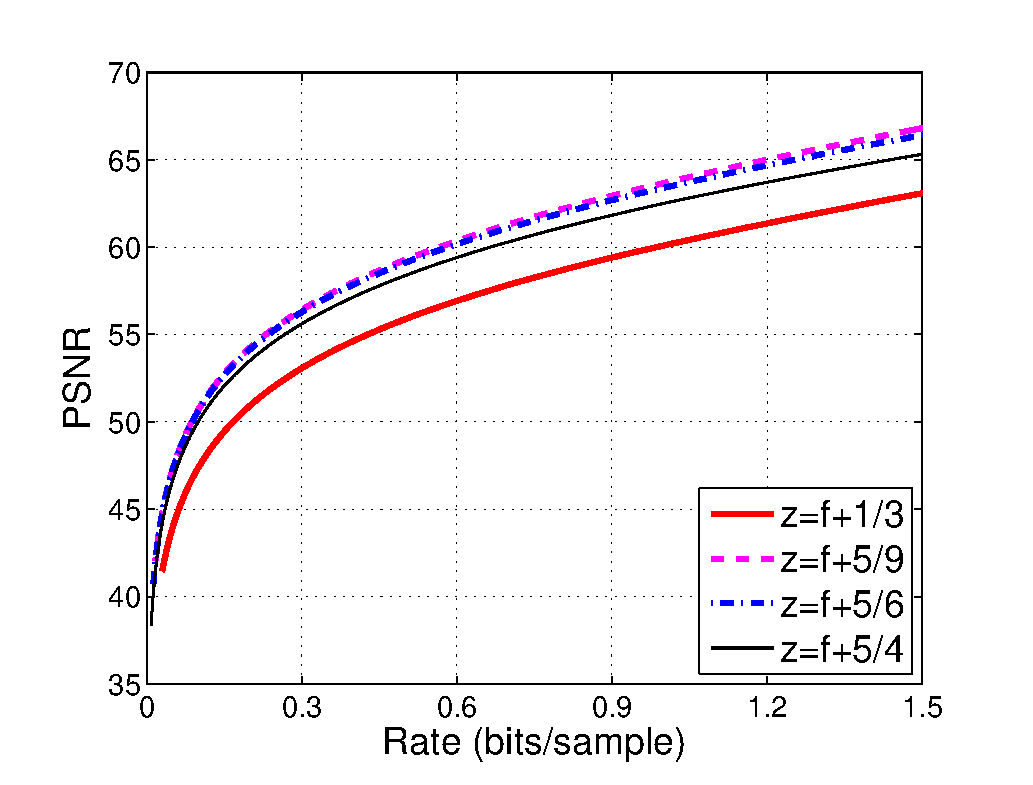
\includegraphics[width = 0.5\linewidth]{Figures/section4/RD_Cauchy_mu=0_2_linear_patterns} &
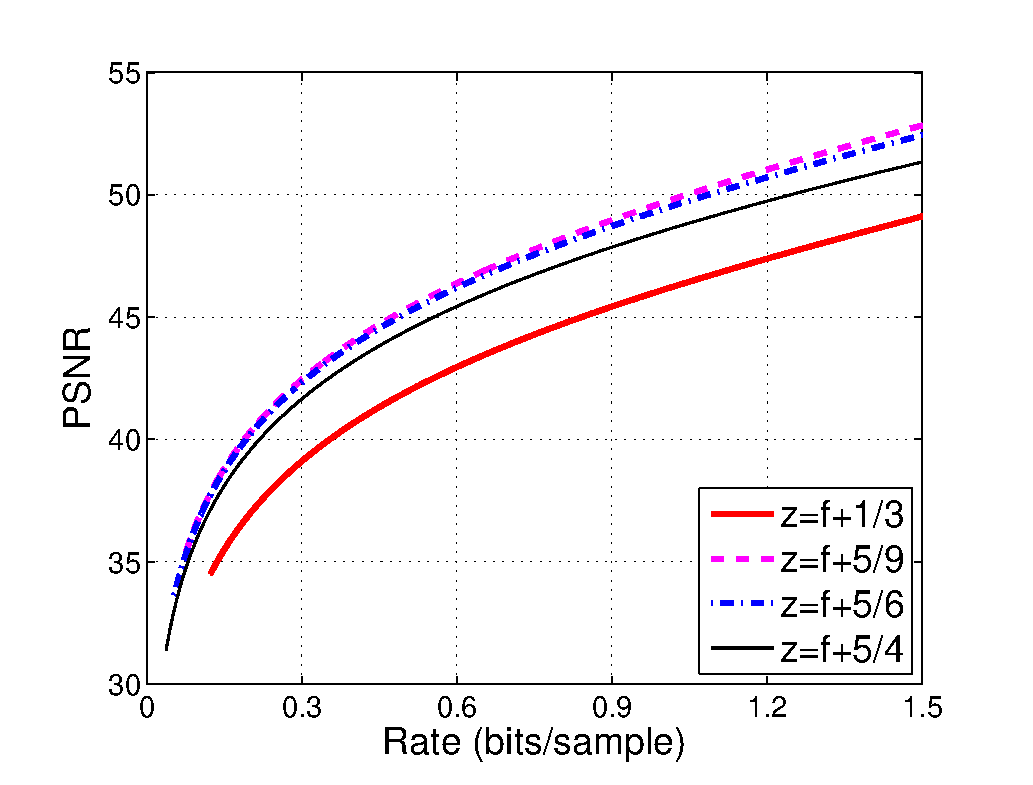
\includegraphics[width = 0.5\linewidth]{Figures/section4/RD_Cauchy_mu=0_8_linear_patterns} \\
{\small (a) Cauchy $\mu=0.2$} & {\small (b) Cauchy $\mu=0.8$}
\end{tabular}
\end{center}
\vspace{-20pt}
\caption{\label{fig:RD_different_patterns}
R-D performance comparison of different DZ+UTSQ/NURQ linear patterns, which reflects the superiority of the patterns satisfying (\ref{equ:formula-LinearConstraint}).}
\end{figure} 

Deduced from the necessary condition (\ref{equ:formula-OptQuant}), in actual bitrate ($0-1.5$ bits/sample), the linear constraint (\ref{equ:formula-LinearConstraint}) is an efficient principle to evaluate the R-D performance of different DZ+UTSQ/NURQ designs, which can be reflected via two groups of simulation experiments on Cauchy distribution. The first group of experiments are designed to show that the linear constraint is a precise performance classifier of DZ+UTSQ/NURQ. Related results for $\mu = 0.5$ are exhibited in Fig. \ref{fig:RD_same_pattern}. From the R-D performance comparison of different DZ+UTSQ/NURQ designs, it is observed that, under each linear pattern, all the PSNR-R curves are exactly overlapped with each other, indicating the identical R-D performance of different DZ+UTSQ/NURQ designs conforming to the same linear pattern satisfying (\ref{equ:formula-LinearConstraint}). The second group of experiments are designed to show that the linear constraint is also an accurate indicator of superior R-D performance. Related results for $\mu = 0.2$ and $0.8$ are exhibited in Fig. \ref{fig:RD_different_patterns}. From the R-D performance comparison of different linear patterns, it is obvious that only the linear patterns satisfying (\ref{equ:formula-LinearConstraint}) can achieve desirable R-D performance.

It should be noted that, as an efficient DZ+UTSQ/NURQ design principle, the linear constraint (\ref{equ:formula-LinearConstraint}) is not only applicable for Cauchy distribution but also for a big class of zero-mean heavy-tailed distributions (requiring monotonic PDF in positive axis). Actually, even for GGD, this constraint is a good R-D performance evaluator, as is shown in our previous work \cite{Sun_TIP2013}. However, since GGD has faster, exponential rate of decay, for GGD, different DZ+UTSQ/NURQ designs conforming to the same linear pattern of $z$ and $f$ may have slight deviation in R-D performance. 

In sum, the constraints (\ref{equ:formula-PreConstraint}), (\ref{equ:formula-RefConstraint}) and (\ref{equ:formula-LinearConstraint}) provide a convenient way to simplify the R-D performance analysis of various different source distributions. Benefiting from these principles, the reason why the DZ+UTSQ/NURQ designs applied in video/image coding standards (e.g. in H.264/AVC, $z$ is set to $2/3$ in intra coding and $5/6$ in inter coding, $f$ is set to $0$ \cite{Sullivan_VCIP2005}) are effective can now be theoretically explained.

\section{Conclusion}
\label{sec:conclusion}

In this paper, universal properties and principles that apply to various source distributions are revealed. First, for any source distribution that can be expressed as the product of a Scaling Factor (SF) and its remaining part, SF does not affect the derivative of its R-D function. Second, for the DZ+UTSQ/NURQ scheme to achieve optimum R-D performance, its parameters should satisfy $\frac{1}{2} \le z - f \le 1$. These results can provide insights and assistance in R-D modeling and quantizer design for real coding applications, regardless of the distribution form of the source. 

\section*{References}
\bibliographystyle{IEEEtran}
\bibliography{refs}

\end{document}
